\chapter{Analýza}\label{chapter:analyza}
% Hlavním cílem této bakalářské práce je implementovat návrh backendu podle návrhu a fragmentu implementace, které byly udělány v rámci předmětů BI-SP1 a BI-SP2 bakalářského studia vyučovaných na FIT ČVUT v akademickém roce 2018/2019 a 2019/2020. 

%TODO move commit footnote to reserse and git footnote
Tato kapitola se zabývá analýzou existujícího návrhu a současného stavu implementace. Pro zajištěni verze aplikace, která bude předmětem analýzy této kapitoly, uvádím datům ukončení práce na projektu v rámci předmětu BI-SP2 -- 25. února 2020. Také pro možnost pohodlného vyhledání konkretní verze  (\url{https://gitlab.fit.cvut.cz/rozvody/be-springboot}), uvádím poslední \texttt{commit}\footnote{proces při kterém se uloží všechny udělané v rámci systému řízení verzí změny a zařadí se do historie změn} udělaný přes distribuovaný systém řízení verzí -- Git -- v rámci tohoto předmětu: 
\begin{quote}
    \enquote{252b0288dbfe9942446b78fd452c0edce810a370}
\end{quote}

\section{Předmět BI-SP1}\label{analyza:navrh:sp1}
    % TODO REST footmote to first mention
    V rámci předměty BI-SP1 pracovalo sedm lidí včetně autora této práci. Tým měl za úkol analyzovat požadavky zákazníka a navrhnout implementaci aplikace. Během semestru tým provedl kompletní analýzu požadavku zákazníka. Především, tým navrhl scénáře použiti aplikace:
    \begin{itemize}
	   \item Přihlašování/Registrace;
	   \item Přihlašování/Registrace do rodiny;
	   \item Role v aplikace a jejich vytváření;
	   \item Nastavení pečovatelský dnů;
	   \item Kalendář;
	   \item Kniha potřeb dítěte;
	   \item Uchování účtenek;
	   \item Správa alimentů.
	\end{itemize}
    Potom byly navrženy diagram užití\footnote{popisuje chování systému z vnějšího pohledu} a diagram aktivit\footnote{zobrazuje jak objekty spolupracují}, podle kterých byly navrženy drátový model pro frontendovou část aplikace a doménový model\footnote{náčrt základních entit systému a vztahů mezi nimi} pro backendovou část aplikace. 
    
    Výsledný návrh aplikace se skládá ze dvou částí. Frontendová část aplikace je reprezentována Android aplikací, kterou současně řeší kolega -- Martin Beran -- v rámci bakalářské práci. Backendová část aplikace, která je předmětem této bakalářské práci, je reprezentovaná serverovým backendem poskytující REST API pro Android aplikaci.

    % Serverového backendu, který je předmětem této bakalářské práci a frontendové částí aplikace, kterou současně řeší kolega -- Martin Beran -- v rámci bakalářské prací. Frontendová část aplikace je Android aplikací. Backendová část je serverovým backendem, poskytujícím REST\footnote{Representational State Transfer} API pro Android aplikaci.

\section{Předmět BI-SP2}\label{analyza:navrh:sp2}
    %TODO gradle footnote to reserse and Spring footnote
    Cílem předmětu BI-SP2 byla implementace návrhu předmětu BI-SP2. Autor této práce pracoval v backendovém týmu a zároveň vystupoval v roli vedoucího backendového týmu.
    
    Pro vývoj backendove částí aplikace byl zvolen jazyk Kotlin, zmíněný v sekci \ref{resere:kotlin}, a framework Spring, zmíněný v sekci \ref{resere:j2ee}. Jako nástroj pro automatizaci sestavování programu byl zvoleny nástroj Gradle. Podrobněji výsledky předmětu BI-SP2 budou probrány v sekci \ref{analyza:soucasnaImplementace}.
        
    
\section{Doménový model}\label{analyza:navrh:DomainModel}
    Hlavním zdrojem informace o výsledném návrhu serveru je doménový model. Kompletní doménový model se nachází v příloze \ref{dodatek:DomainModel}. Během implementace tým označoval entity, které jsou kompletně nebo částečně implementovány. Zelenou barvou jsou označeny třídy, které už jsou implementovány. Žlutou barvou jsou označeny třídy, které ještě nejsou implementovány. Také, jsou třídy označeny zároveň žlutou a zelenou barvou, což znamená, že třída je implementována jenom částečně. Taková situace se mohla nastat v případe, že implementace vyžadovala implementaci jiné třídy, která ještě neexistovala. Tento doménový model má nedostatky detekované při implementaci, jak frontendové, tak i backendové částí aplikace. Jako příklad takových nedostatků je možné uvést zbytečně komplikovaný návrh entity \texttt{Interval} (viz obrázek \ref{image:Interval1}). Podrobný popis problému bude uveden v sekci \ref{analyza:pozadavky-frontendu}.

\section{Analýza současného návrhu} \label{analyza:analyza navrhu}
    V této sekci budou podrobně popsány klíčové aspekty aplikace podle současného návrhu. Problémy a navržené změny těchto částí budou popsány v následujících sekcích.

    \subsection{Registrace a přihlášeni do systému}
        Aplikace je navržena takovým způsobem, že první uživatel, který má vytvořit svůj účet je jeden z rodičů. Pro registraci člověk potřebuje řadu povinných údajů:
        \begin{itemize}
	        \item jméno -- zvolené jméno se stává jeho implicitním jménem v systému;
	        \item příjmení -- zvolené příjmení se stává jeho implicitním příjmením v systému;
	        \item poštvou adresu -- zvolený email je identifikátorem uživatele v rámci systému;
	        \item heslo -- heslo pro autorizaci v systému.
        \end{itemize}
        Na základe těchto údajů se vytvoří unikátní uživatel v rámci systému. V tento okamžik člověk není přihlášen do žádné rodiny a nemá žádnou roli. Podrobněji role budou popsané v sekci \ref{analyza:bezpecnost:role}.
        % \begin{figure}\centering
	       % 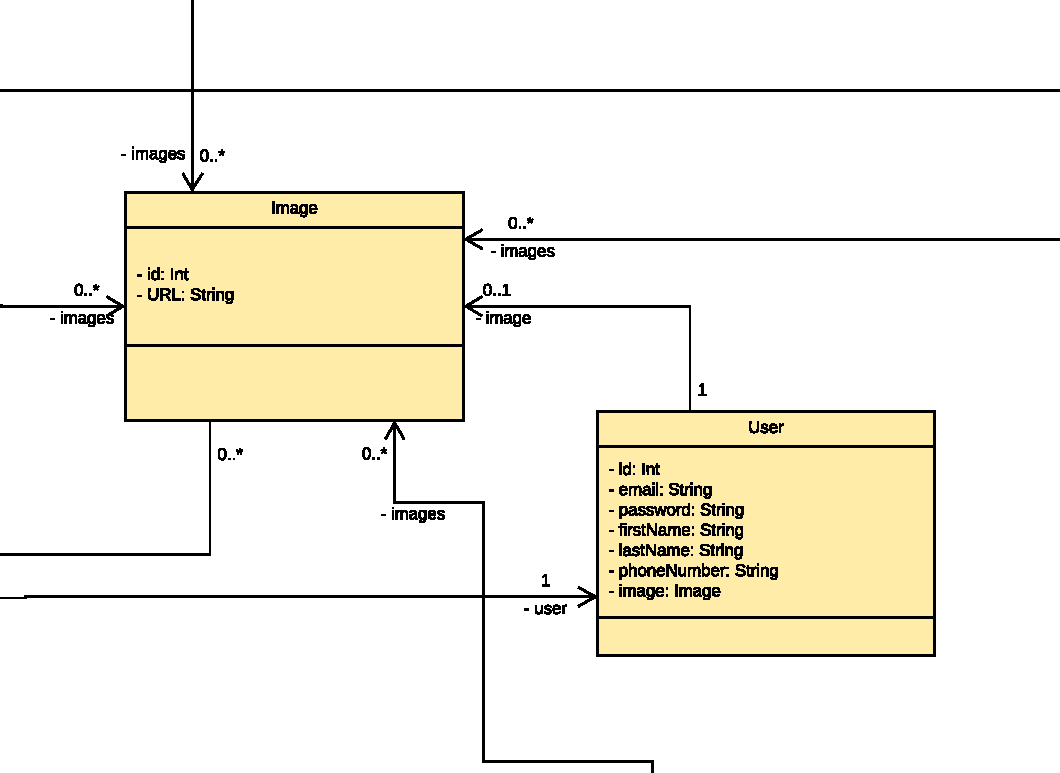
\includegraphics[width=0.7\textwidth]{pdfs/User-Image1}
	       % \caption[Návrh User-Image]{Vztah mezi třídami \texttt{User} a \texttt{Image} podle Doménového modelu z předmětu BI-SP2}\label{image:User-Image1}
        % \end{figure}
        
        Potom uživatel má možnost vytvořit rodinu nebo přihlásit se do již existující rodiny. Pro vytvoření nové rodiny, uživatel potřebuje zadat jméno rodiny a přidat členy rodiny. Autor této rodiny automaticky se stává jedním s rodičů této rodiny. Jinou možností je se přihlásit do rodiny, která již existuje. Podmínkou je existování pozvání do některé existující rodiny, což znamená, že přidat nového uživatele do rodiny může jenom člen této rodiny. V takovém případě uživatel už nemá možnost zvolit role v rámci rodiny. Role má být nastavena uživatelem, který vytvořil toto pozvání.

    \subsection{Kalendář}    
        Kalendář je hlavním zdrojem informace pro celou rodinu a je společný pro všechny uživatele. Na něm jsou zobrazené zvýrazněné různými barvami pečovatelské dny obou rodičů. Také, kalendář zobrazuje jednorázové a pravidelné události.
        
        \begin{figure}\centering
	        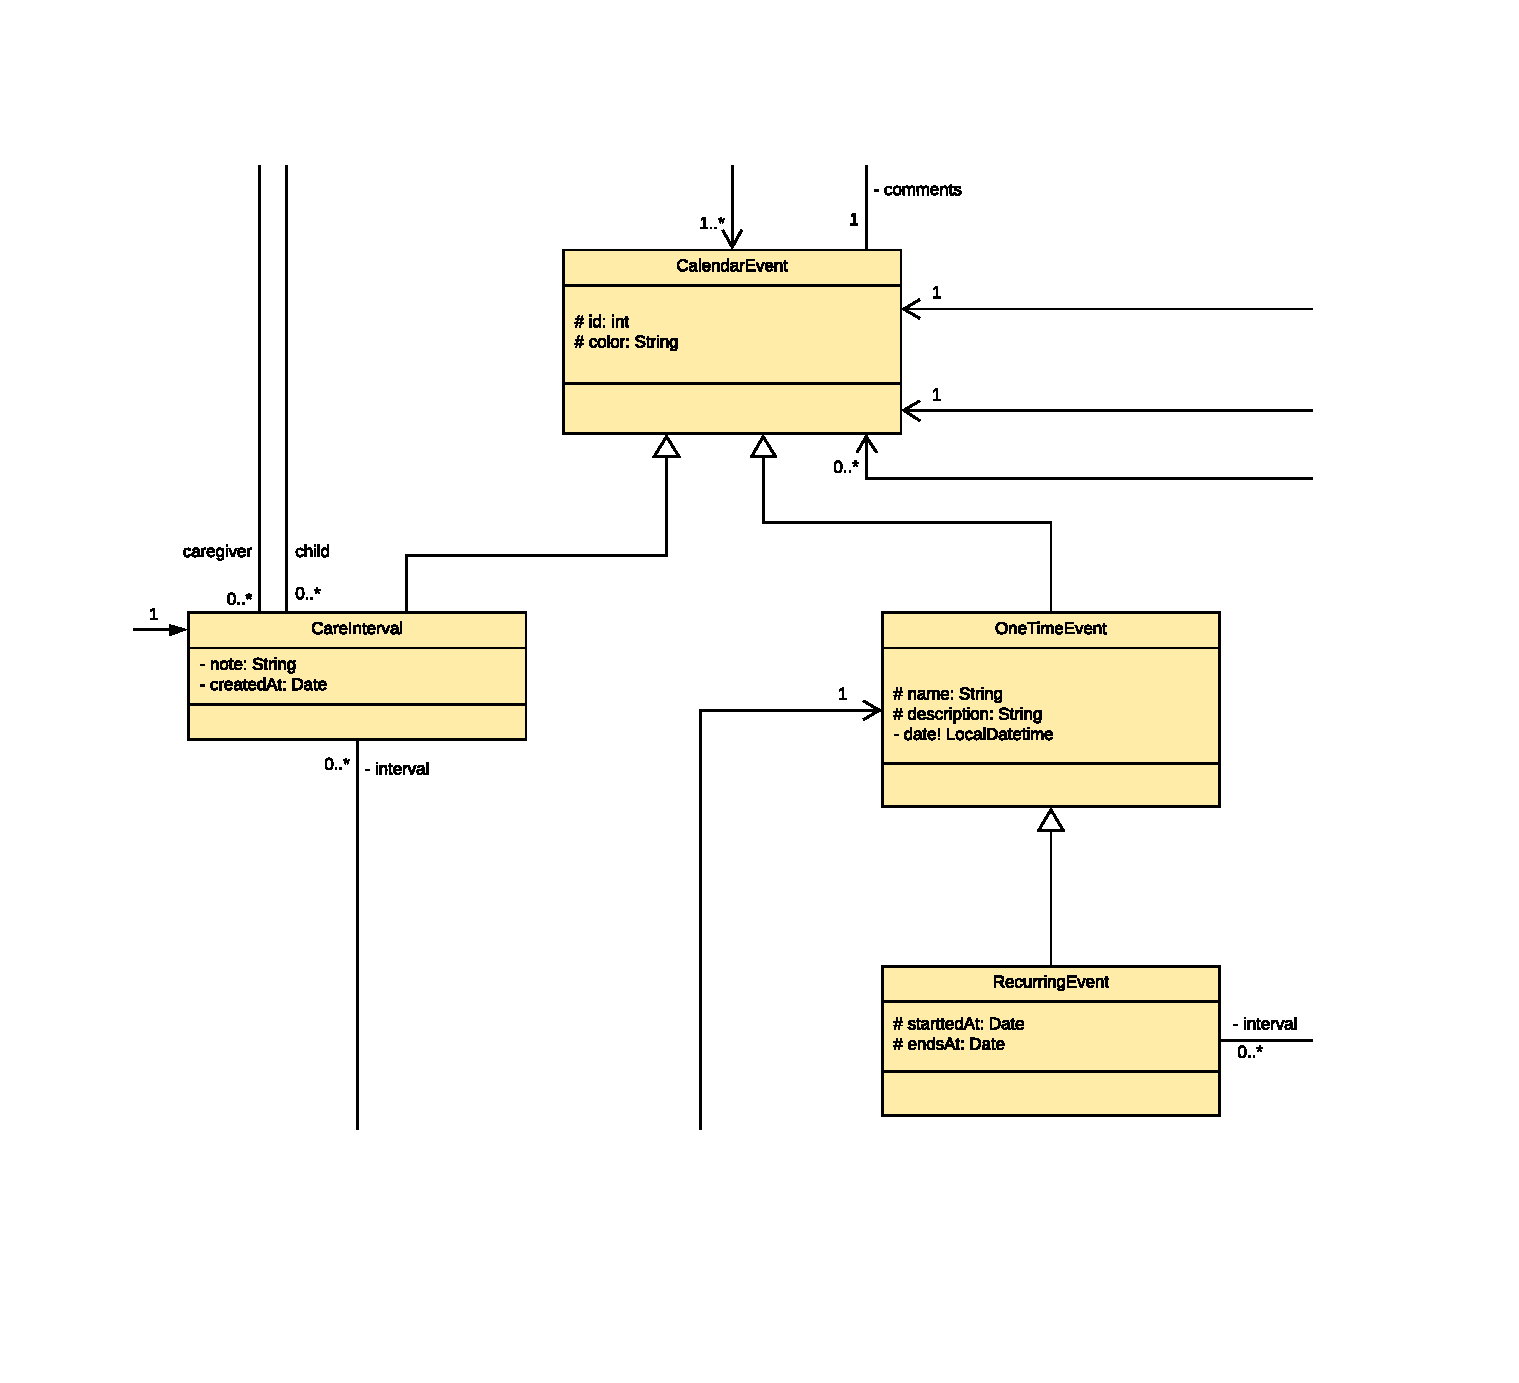
\includegraphics[width=1.0\textwidth]{pdfs/CalendarInfo1}
	        \caption[Současný návrh kalendáře]{Návrh kalendáře podle doménového modelu z předmětu BI-SP2}\label{image:calendar-info}
        \end{figure}
        Doménový model neobsahuje informaci o kalendáři, ale obsahuje entity reprezentující informaci, kterou kalendář bude zobrazovat (viz obrázek \ref{image:calendar-info}). Každý element, který bude zobrazen v kalendáři, je reprezentován stejnou entitou \verb|CalendarEvent|. Entita obsahuje jenom informaci o barvě, kterou událost bude zobrazená v kalendáři a závislost na entitu \verb|Comment|. Za reprezentaci pečovatelských dnů odpovídá entita \verb|CareInterval|, která se dědí od entity \verb|CalendarEvent|. Za reprezentaci jednorázových a opakujících se události odpovídají entity \verb|OneTimeEvent| a \verb|RecurringEvent|, kde \verb|RecurringEvent| se dědí od \verb|OneTimeEvent|.
        
        % Současný návrh kalendáře nepokrývá všechny scénáře použití. Podrobný popis problémů a navržené změny budou uvedeny v sekci \ref{analyza:kalendar}. 
        
        % Kromě dlouhodobých nastavení pečovatelských dnu, kalendář může zobrazovat i jednorázové změny, které mohou vidět všechny členy rodiny. 
    \subsection{Alimenty}
        \begin{figure}\centering
	        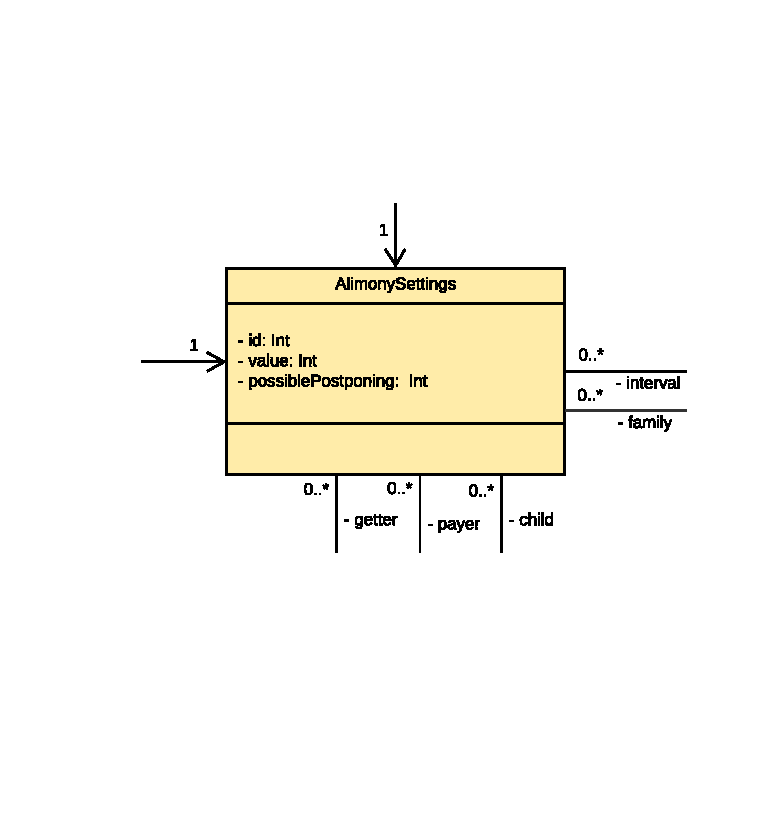
\includegraphics[width=0.7\textwidth]{pdfs/AlimonySettings1}
	        \caption[Návrh entity \texttt{AlimonySettings}]{Návrh entity \texttt{AlimonySettings} podle doménového modelu z předmětu BI-SP2}\label{image:AlimonySettings1}
        \end{figure}
        \begin{figure}\centering
	        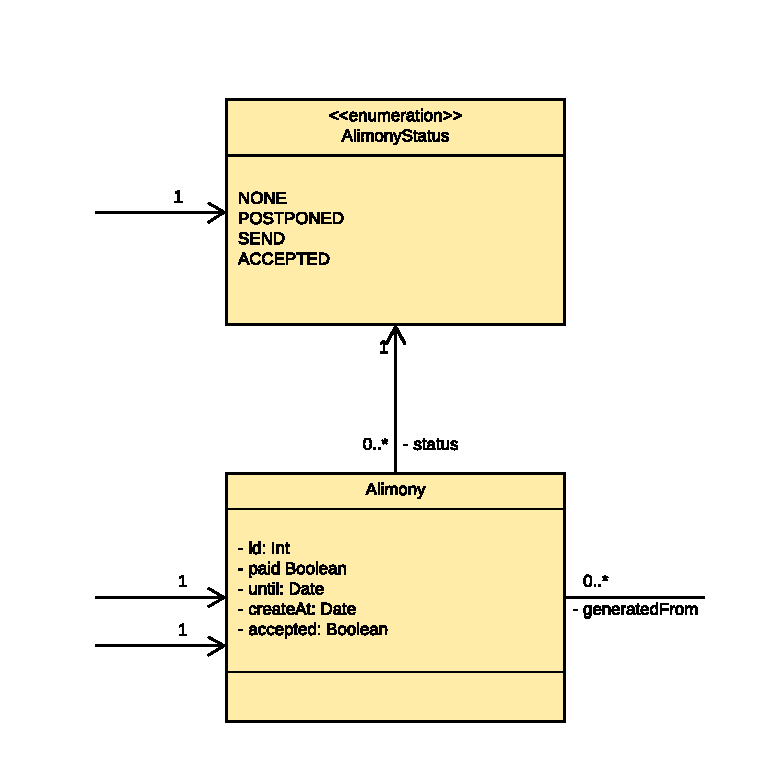
\includegraphics[width=0.7\textwidth]{pdfs/Alimony1}
	        \caption[Návrh entity \texttt{Alimony}]{Návrh entity \texttt{Alimony} podle doménového modelu z předmětu BI-SP2}\label{image:Alimony1}
        \end{figure}
        Důležitou částí aplikace je správa alimentů, které má pravidelně uhrazovat jeden z rodičů. Tento proces byl rozdělen do dvou částí. První částí je dlouhodobé nastavení alimentů (viz obrázek \ref{image:AlimonySettings1}). Druhou částí jsou samotné alimenty (viz obrázek \ref{image:Alimony1}), které se generuje na základě dlouhodobých nastavení. Jedna rodina může mít zároveň několik nastavení v případě, že jedna rodina má několik dětí nebo chce rozdělit alimenty do logických bloků.
        
        Každá instance alimentů má stav, který se postupně mění. V moment vytvoření instance má stav \verb|NONE|. Po odesílání alimentů druhému rodiči, stav se mění na \verb|SEND|. Potom druhý rodič má potvrdit, že alimenty přijal, a tím změnit stav na \verb|ACCEPTED|. Také se může nastat situace, kdy rodič nemá možnost odeslat alimenty včas, což se může nastat z různých důvodů. V takovém případě stav instanci se mění na \verb|POSTPONED|.
    
    \subsection{Kniha potřeb dítěte}\label{analyza:navrh:need}
        \begin{figure}\centering
	        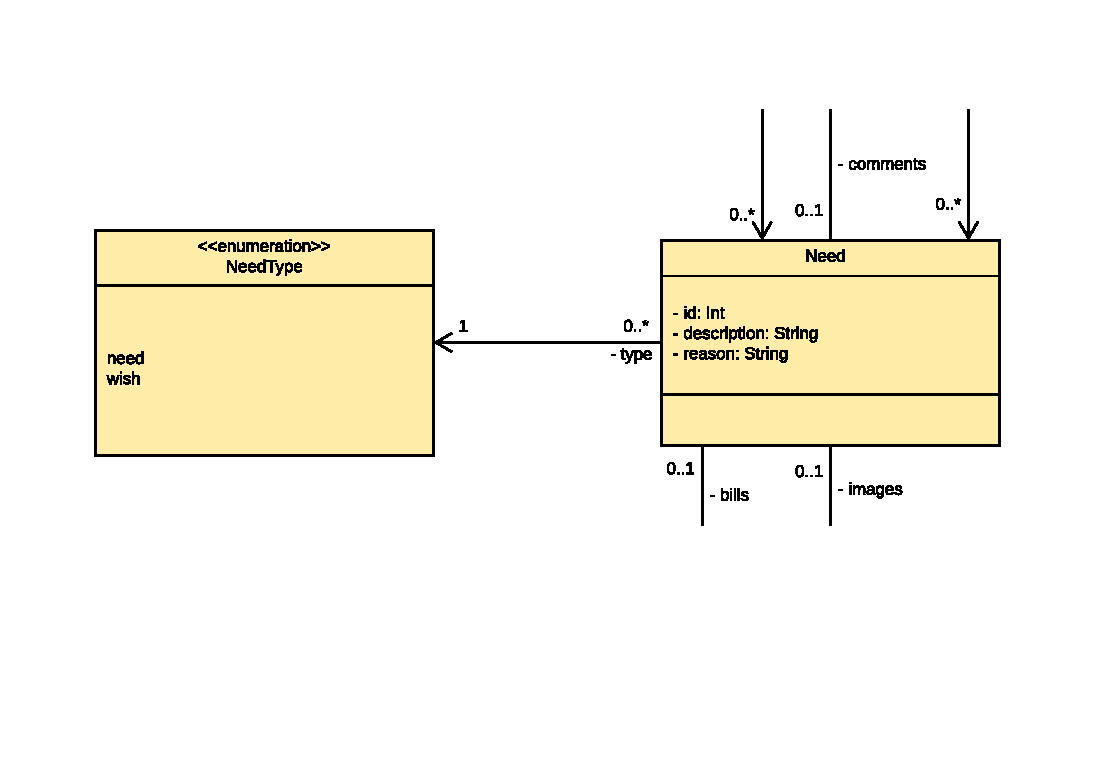
\includegraphics[width=0.9\textwidth]{pdfs/Need1}
	        \caption[Návrh \texttt{Need}]{Návrh entity \texttt{Need} podle doménového modelu z předmětu BI-SP2}\label{image:Need1}
        \end{figure}
        Jedním s populárních problémů, které vznikají během procesu rozvodu, je nakupování příliš drahých dárku o kterých nevědí ostatní členy rodiny. Jako příklad je možné uvést nakupování bot pro dítě. Jeden s rodičů může chtít \enquote{koupit lásku dítěte} a koupit několikrát dražší boty než dítě opravdu potřebuje. Kniha potřeb dítěte (viz obrázek \ref{image:Need1}) je zaměřena na překonání takových situací.
        
        \begin{figure}\centering
	        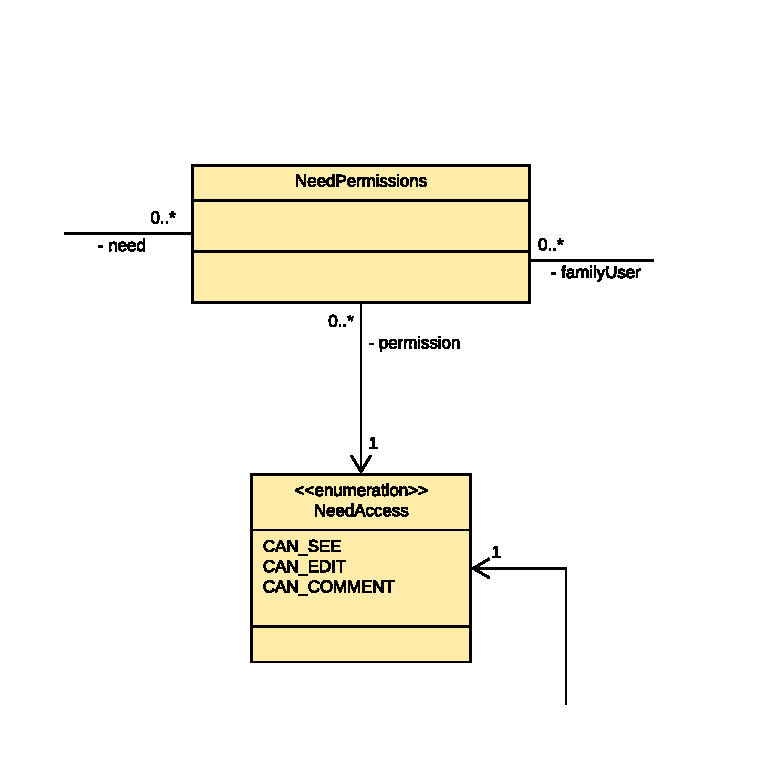
\includegraphics[width=0.8\textwidth]{pdfs/NeedPermissions1}
	        \caption[Návrh entity \texttt{NeedPermissions}]{Návrh entity \texttt{NeedPermissions} podle doménového modelu z předmětu BI-SP2}\label{image:NeedPermissions1}
        \end{figure}
        Potřeba může být typu \verb|need| nebo \verb|wish|. Podle současného návrhu je rozdíl mezi typy pouze pro informační účely. Každé instanci entity \verb|Need| patři instance entity \verb|NeedPermission| (viz obrázek \ref{image:NeedPermissions1}), která definuje přístupová práva pro jednotlivé členy rodiny. V případě, že uživatel nemá žádné z přístupových práv, potřeba se nevyskytuje v jeho seznamu potřeb dítěte. Toto pravidlo se netýká jenom rodičů, které mají přistup ke všem potřebám automaticky.
       
       Potřeba obsahuje následující informaci:
        \begin{itemize}
            \item popis -- popis potřeby;
            \item příčina -- příčina proč dítě tohle potřebuje;
            \item obrázky -- obrázky věcí, kterou dítě potřebuje;
            \item účtenky -- účtenky v případě, že někdo z rodičů splnil potřebu;
            \item komentáře -- komentáře členu rodiny včetně dítěte.
        \end{itemize}
    
    \subsection{Účtenky}
        \begin{figure}\centering
	        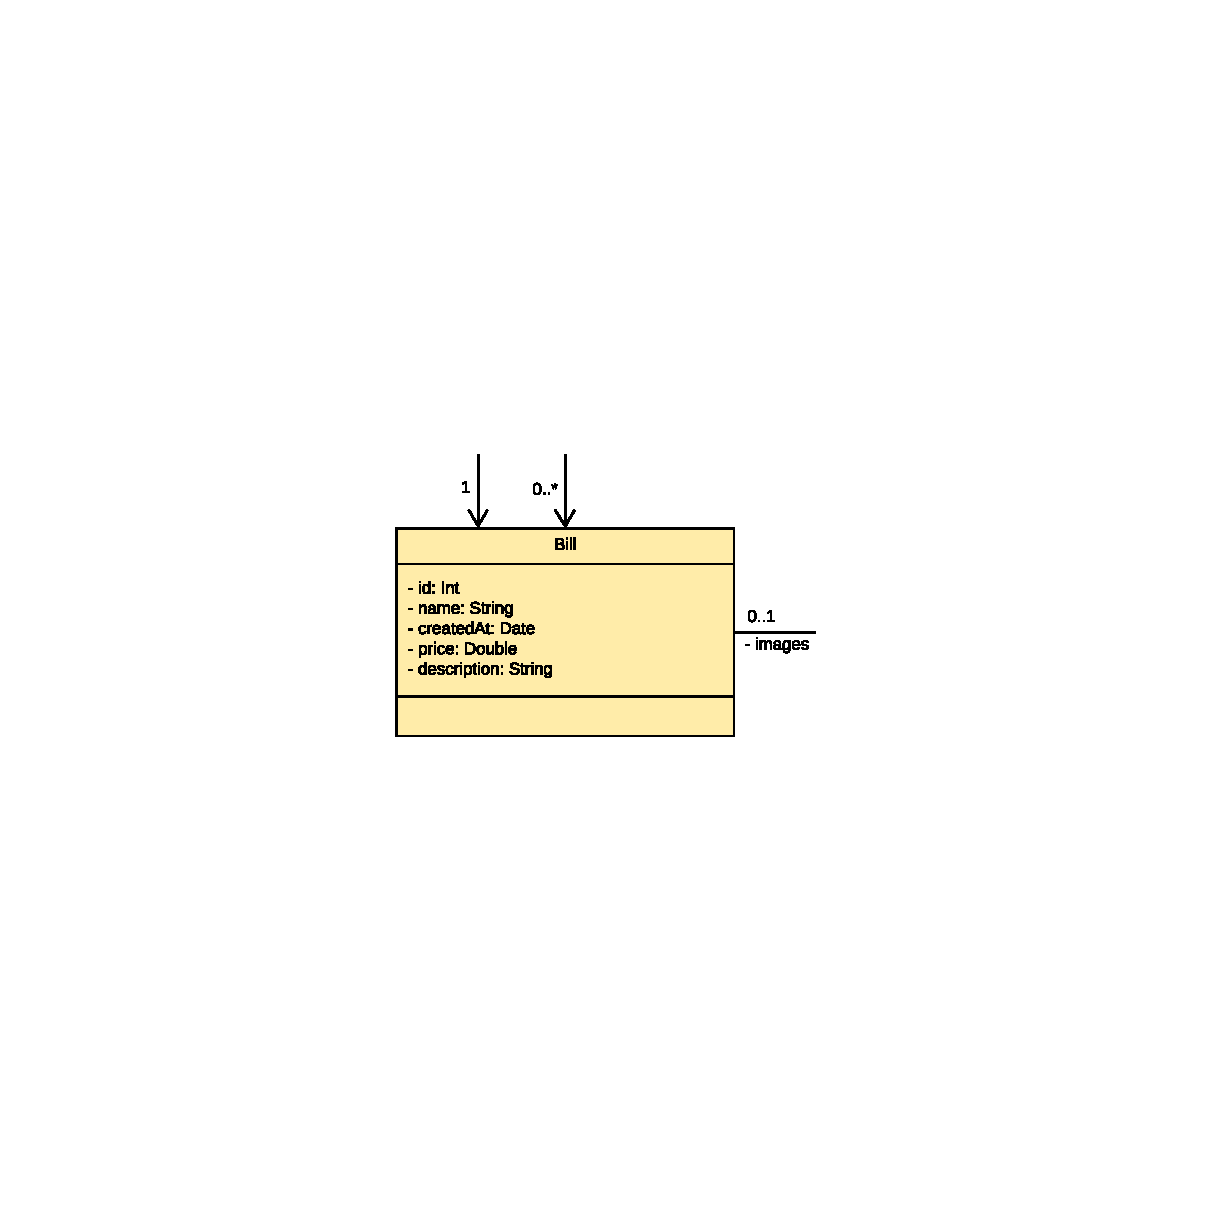
\includegraphics[width=0.6\textwidth]{pdfs/Bill1}
	        \caption[Návrh entity \texttt{Bill}]{Návrh entity \texttt{Bill} podle doménového modelu z předmětu BI-SP2}\label{image:bill1}
        \end{figure}
        V sekci \ref{analyza:navrh:need} už bylo zmíněno, že je potřeba řešit problém nakupování dárku pro dítě, ale kniha potřeb dítěte řeší tenhle problém jenom částečně. Nikdo nezabraní uživateli uvést v popisu splněného požadavku nebo potřeby neplatné údaje, proto byla zavedena možnost přidání účtenky (viz obrázek \ref{image:bill1}). Tato entita, kromě údajů o nakoupeném zboží, umožňuje přidání fotografií potvrzujících platnost uvedených údajů.
    
    \subsection{Požadavky na změny}
        Každý člen rodiny může udělat určité změny v rámci rodiny. Například nastavit přezdívku pro konkretního uživatele nebo přidat fotografii do události v kalendáři. Každá taková změna je důležitá, ale jsou změny, které by měly být kontrolovány rodiči. Pro zaručení kontroly byly zavedeny požadavky na změny pro některé změny v rámci rodiny:
        \begin{itemize}
            \item \texttt{AlimonySettingRequest} -- požadavek na změnu nastavení alimentů, který může být vytvořen jedním z rodičů;
            \item \texttt{AlimonyChangeRequest} -- požadavek na změnu stavu instance alimentů, který může být vytvořen jedním z rodců;
            \item \texttt{OneTimeEventRequest} -- požadavek na vytvoření jednorázové události v kalendáři, který může být vytvořen libovolným cleném rodiny;
            \item \texttt{OneTimeEventChangeRequest} -- požadavek na změnu již existující události v kalendáři, který může být vytvořen libovolným členem rodiny;
            \item \texttt{ChildItemRequest} -- požadavek na změnu nastavení pečovatelských dnů, který může být vytvořen libovolným členem rodiny. Změna může být, jak jednorázová, tak i dlouhodobá.
        \end{itemize}
        \begin{figure}\centering
	        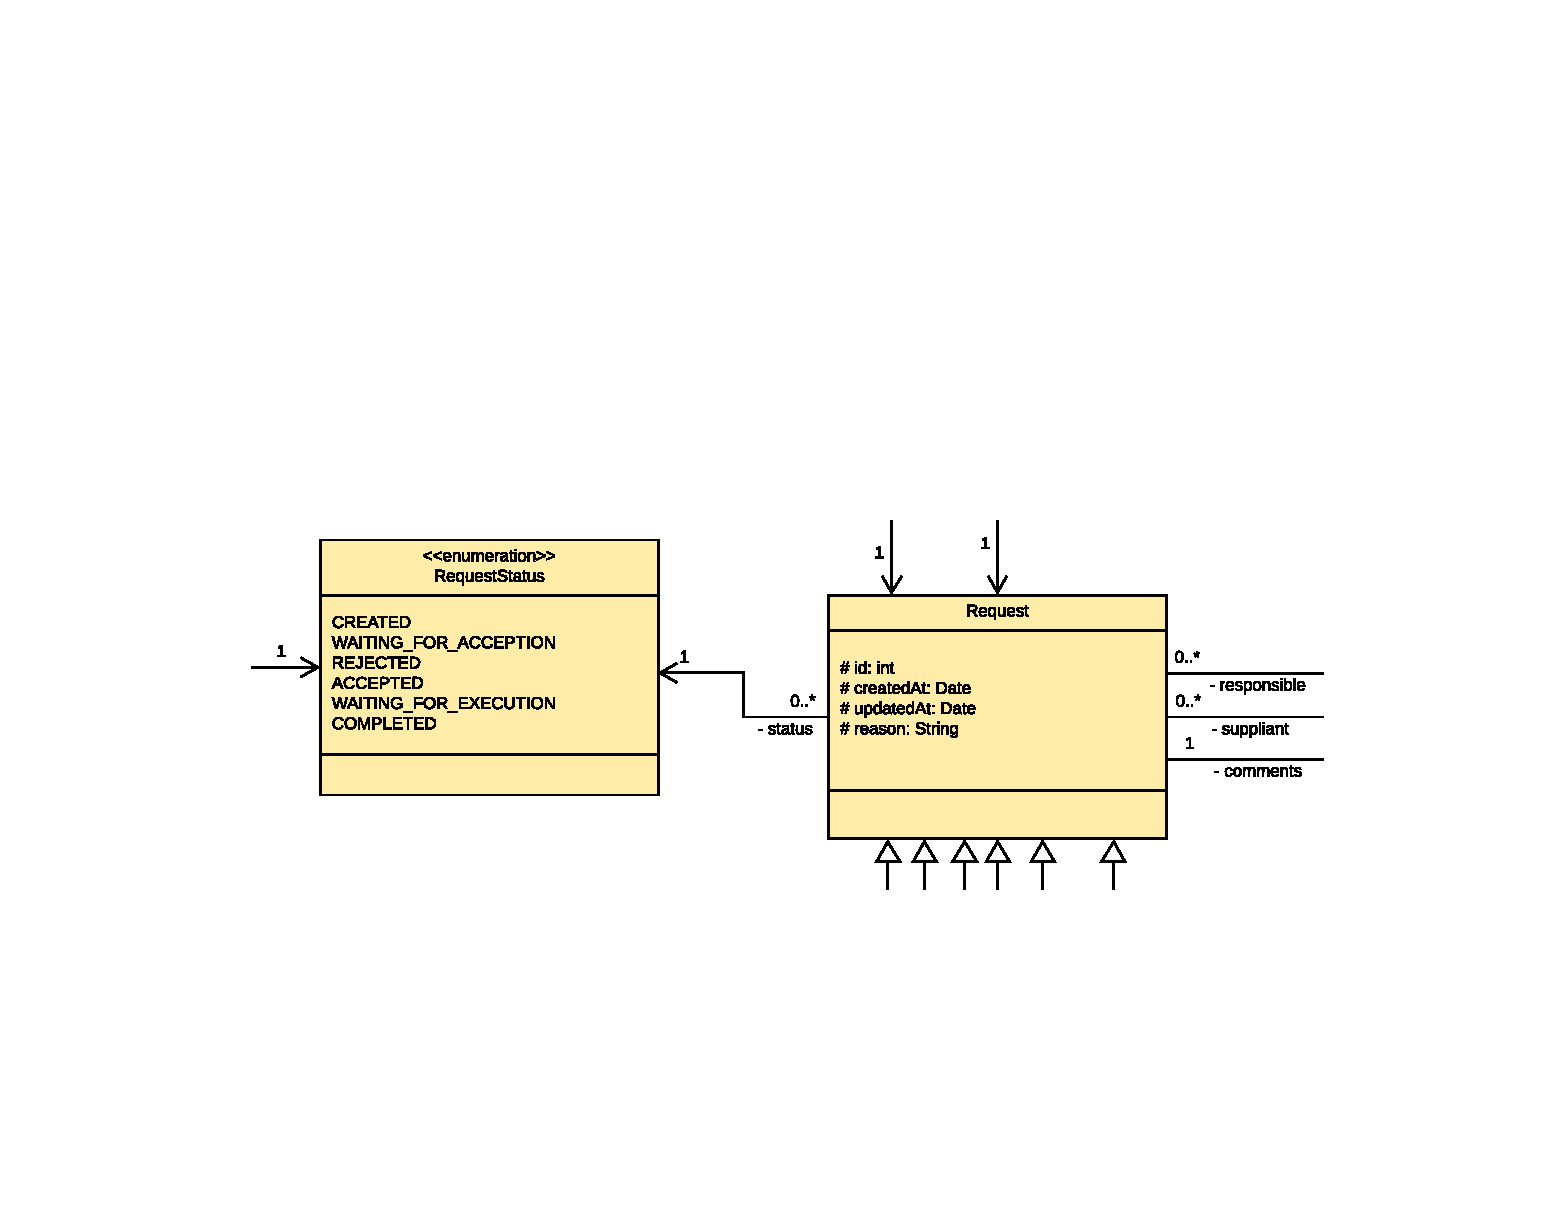
\includegraphics[width=0.9\textwidth]{pdfs/Abstr-Requrest1}
	        \caption[Návrh abstraktní entity \texttt{Request}]{Návrh abstraktní entity \texttt{Request} podle doménového modelu z předmětu BI-SP2}\label{image:abstr-request1}
        \end{figure}
        Každá entita požadavku je zděděna od společné abstraktní entity obsahující základní informace o požadavku (viz obrázek \ref{image:abstr-request1}). Mezi základními informacemi patří datum vytvoření, datum poslední změny, příčina a také aktuální status požadavku.
        
        Statusy požadavků reprezentují jejích životní cyklus. Při vytvoření každý požadavek má stejný status -- \verb|CREATED|. Po zveřejnění, požadavek má status \verb|WAITING_FOR_ACCEPTING|. Po schváleni, status se mění na \verb|ACCEPTED| nebo na \verb|WAITING_FOR_EXECUTION| v případě, že změna je akceptována, ale ještě není uplatněna. Také může nastat případ, že požadavek byl zamítnut, potom status se mění na \verb|REJECTED|. V okamžik, kdy požadavek je schválen nebo se čeká na uplatnění, už není možné měnit položky tohoto záznamu. Právo na schválení nebo zamítnutí požadavků mají jenom rodiče. Požadavky, které byly vytvořeny jedním z rodičů, mají být potvrzeny druhým rodičem. Ostatní požadavky musí být potvrzeny oběma rodiči.
    
    \subsection{Historie změn}
        Podle požadavků zákazníka, všechny změny v rámci rodiny by měly být zaznamenány. Proto byly zavedeny entity historií, které kopírují všechny položky entit a přidávají datum vytvoření záznamu a odkaz do patřičné entity v případě, že táto příslušná entita byla aktualizována. Takové entity jsou zavedeny jenom pro důležité části aplikace, které se mohou měnit uživatelem:
        \begin{itemize}
            \item \texttt{CalendarEventHistory};
            \item \texttt{BillHistory};
            \item \texttt{AlimonyHistory};
            \item \texttt{AlimonySettingsHistory};
            \item \texttt{RequestHistory}.
        \end{itemize}
        Všechny typy historie jsou zděděny od stejné entity -- \verb|History|. Tato entita obsahuje základní údaje pro libovolný typ historie: ID\footnote{identifikátor} a datum vytvoření záznamu. 
     
\section{Analýza současné implementace}\label{analyza:soucasnaImplementace}
    \begin{figure}\centering
	   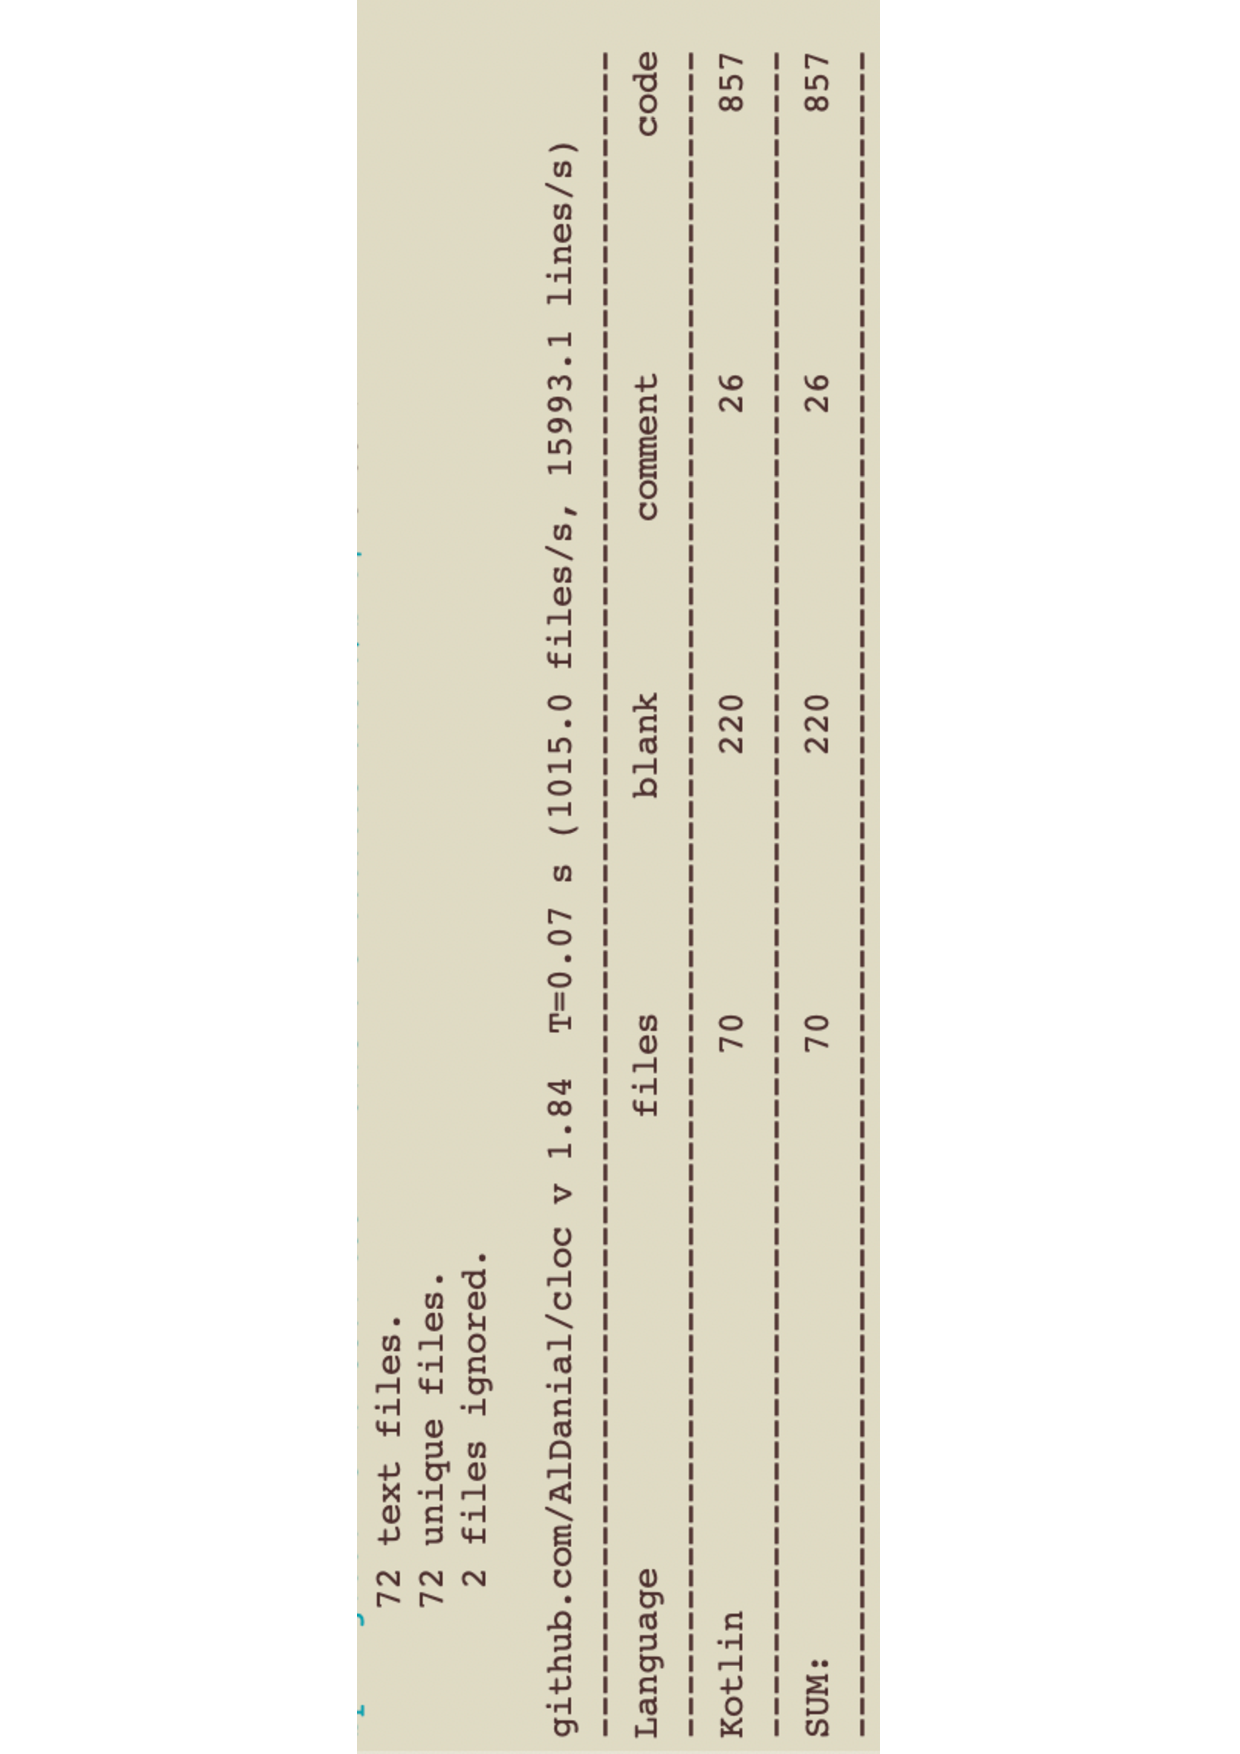
\includegraphics[angle=-90, width=0.9\textwidth]{pdfs/Cloc1}
	   \caption[Počet řádků kódu před začátkem práce]{Počet řádků kódu před začátkem práce}\label{image:cloc1}
    \end{figure}
    Současná implementace obsahuje 69 souborů a 845 řádek kódů (viz~obrázek~\ref{image:cloc1}). Práce byla provedena členy týmu předmětu BI-SP2 vyučovaného na FIT ČVUT v Praze. Za účelem zvětšení přesnosti analýzy byl zvolen nástroj pro analýzu počtu řádek kódu, který byl popsán v sekci \ref{reserse:cloc}. Implementace částečné pokrývá doménový model zmíněný v sekci \ref{analyza:navrh:DomainModel}. V této sekci budou popsány již implementované části aplikace. 
     
    Pro implementaci serverového backendu byla zvolena architektura REST skládající se ze tří vrstev:
    \begin{itemize}
         \item Aplikační vrstvy, která pokrývá scénáře využiti aplikace;
         \item Doménové vrstvy, která obsahuje logiku aplikace;
         \item Datové vrstvy, která komunikuje s databází.
    \end{itemize}
    
    Pro implementaci datové vrstvy byl použit framework Spring Data, který byl popsán v sekci \ref{resere:j2ee}. Nástroj přidává dodatečnou vrstvu pro implementaci JPA a tím zrychluje a zjednodušuje implementaci. Pro implementaci této vrstvy bylo zvoleno rozhraní \verb|CrudRepository|, které vyžaduje uvedení typu doménové třídy a typu identifikátoru. Každé entitě patří jedna taková třída pro práci s databází.
    
    Pro implementaci doménové vrstvy byly pro každou entitu přidány rozhraní reprezentující funkci, které je možné provádět s příslušnou entitou. Implementace byla oddělená od definicí metod pro zvětšení modularity výsledného softwaru. Implementace této vrstvy přímo komunikuje s datovou vrstvou. Provázání tříd se vzniká na základě vkládání závislostí. Proces vkládaní řídí framework Spring podle principu IoC. Tato vrstva komunikuje s datovou vrstvou pomocí reprezentací entit, ale s aplikační vrstvou komunikuje pomocí DTO\footnote{data transfer object}. Konverzace s entity na DTO se provádí v příslušné třídě entity. Konverzace s DTO na entitu se provádí v příslušné třídě DTO.
    
    % http requests https://www.ibm.com/support/knowledgecenter/SSGMCP_5.2.0/com.ibm.cics.ts.internet.doc/topics/dfhtl21.html
    Aplikační vrstva je reprezentována sadou řadičů(\textit{controllers}), kde každý řadič je určen pro konkretní aspekt použití aplikace. Například, řadič existuje řadič určený pro práci s entitou \verb|Bill| nebo řadič pro ověření jestli aplikace funguje. Pro každý řadič je vymezená samostatná cesta, která se zadává jako řetězec požadavku\cite{http-request-components}. Tato vrstva přímo komunikuje s doménovou vrstvou. Provázání tříd se provádí také pomocí vkládaní závislostí. Komunikace aplikační vrstvy přes API se provádí pomocí DTO.
    
    \subsection{Implementované entity}\label{analyza:implementace:tridy}
        Seznam implementovaných entit:
        \begin{itemize}
            \item \texttt{AlimonyStatus};
            \item \texttt{Bill};
            \item \texttt{CalendarEvent};
            \item \texttt{OneTimeEvent};
            \item \texttt{Comment};
            \item \texttt{FamilyMember} -- je přítomná jenom část implementace;
            \item \texttt{History};
            \item \texttt{IntervalType};
            \item \texttt{NWeekInterval};
            \item \texttt{WeekInterval};
            \item \texttt{NeedAccess};
            \item \texttt{NeedType};
            \item \texttt{AbstractPermissions};
            \item \texttt{Permissions};
            \item \texttt{RequestStatus};
            \item \texttt{User}.
        \end{itemize}
        
        \begin{table}\centering
	    \caption[Konfigurace našeptavače pro řadiče]{Ukázka konfigurace našeptavače zachycování výjimek pro řadiče}\label{tab:excpetion-handler1}
	    \begin{tabular}{|l|c|c|c|}\hline
		  Typ chyby		& HTTP status		& zpáva	& URL	\tabularnewline \hline \hline
		  \texttt{Illegal Access}	& 401	& původní zpráva chyby		& původní cesta     \tabularnewline \hline
		  \texttt{Illegal Argument}	& 400	& původní zpráva chyby		& původní cesta     \tabularnewline \hline
		  \texttt{Null Pointer}	& 500	& původní zpráva chyby		& původní cesta     \tabularnewline \hline
		  \texttt{No Such Element}	& 404	& nic		& nic     \tabularnewline \hline
	    \end{tabular}
        \end{table}
        Kromě kostry aplikace, která zaručuje třívrstvou architekturu, byly také implementovány pomocné třídy zlepšující výsledný návrh aplikace. Jednou z takových tříd je třída, která uvádí nápovědy pro všechny řadiče ohledně zachycování výjimek. Tato třída byla zavedena za účelem poskytování uživateli jenom korektně formátované informace a filtrování zbytečné informace pro koncového uživatele. Konfigurace našeptavače je uvedena v tabulce \ref{tab:excpetion-handler1}. Jiný pomocnou třídou je řadič určeny pro ověření jestli server funguje. Tento řadič je namapován na cestu \enquote{/}.
        
        % Byl přidán \texttt{controller}\footnote{vrstva controlleru zajišťuje REST API komunikaci, překládá výjimky na HTTP kóda zajišťuje omezení pro jednotlivých uživatelů} pro testování, zda aplikace běží, který je namapován\footnote{přidání konkrétnímu controlleru adresy pomocí anotací frameworku Spring, která se zadává jako URI při odesílaní požadavků na Server} na cestu \enquote{/}. Také, byla přidaná třída, která obsahuje nápovědy pro ostatní \texttt{controllery} ohledně zachycování chyb. Tato třída byla zavedena za účelem poskytování uživateli jenom korektně formátovanou informaci  a filtrování zbytečné informace pro koncového uživatele (viz tabulku \ref{tab:excpetion-handler1}). 
        
    
    \subsection{Dokumentace API}
        \begin{figure}
            \begin{minted}
        [frame=lines,
        framesep=2mm,
        baselinestretch=1.2,
        fontsize=\footnotesize,
        linenos]{java}
@Configuration
@EnableSwagger2
class SwaggerConfig {
@Bean
fun api(): Docket {
    return Docket(DocumentationType.SWAGGER_2)
        .select()
        .apis(RequestHandlerSelectors.any())
        .paths(PathSelectors.any())
        .build()
    }
}
            \end{minted}
            \caption{Ukázka nastavení frameworku Swagger}\label{code:swagger-configuration}
        \end{figure}
        
        Pro dokumentaci API byl zvolen framework Swagger, který byl popsán v sekci \ref{resere:dokumentace}. V současné implementaci je použitá druha verze tohoto frameworku. Také byla provedena konfigurace pro generování dokumentace při každém spouštění aplikace na základě přidaných do kódu anotací (viz obrázek \ref{code:swagger-configuration}). Po spuštění aplikace, online dokumentace je dostupná na cestě \enquote{/swagger-ui.html}
    
        % Bylo provedeno nastavení frameworku Swagger pro dokumentace API (viz obrázek \ref{code:swagger-configuration}). Podrobněji framework Swagger byl popsán v sekci \ref{resere:dokumentace}. Po spuštění serveru, dokumentace se automaticky generuje a je přístupná ze stejného portu na cestě \enquote{/swagger-ui.html}.

    \subsection{Profily}\label{analyza:soucasnaImplementace:profily}
    %spring profiles: https://docs.spring.io/spring-boot/docs/current/reference/html/spring-boot-features.html#boot-features-profiles
    %applicatioon peoperties: https://docs.spring.io/spring-boot/docs/current/reference/html/spring-boot-features.html#boot-features-external-config-application-property-files
        Framework Spring, použitý v současné implementaci, poskytuje možnost rozdělit aplikaci do logických bloků, které budou existovat jenom v konkrétních profilech\cite{spring-profile}. Implicitně všechny komponenty nezávisí na aktuálně zvoleném profilu. Pro zavedení profilů\footnote{jedna komponenta může současně patřit několika různým profilům} pro konkretní komponentu je potřeba ji označit anotací \texttt{Profile}. V závorkách vedle anotací je potřeba přidat seznam profilů, ve kterých tato komponenta bude existovat. Konfigurace aktuálně zapnutých profilů se provádí pomocí souboru \texttt{application.properties}, který definuje proměnné pro prostředí aplikace. Soubor se nachází ve složce s cestou \enquote{be-springboot/src/main/resources}.
    
        Každý profil také může obsahovat vlastní konfigurační soubor, který definuje všechny nutné proměnné prostředí. Soubor má byt zadán ve formátu \texttt{application-\{profile\}.properties}, kde \texttt{profile} je názvem profilu kterému patří tento soubor. Současný návrh aplikace obsahuje dva konfiguračních souboru.
    
        První konfigurační soubor obsahuje implicitní proměnné pro prostředí aplikace. Aktuálně soubor má jenom definici aktuálního profilu aplikace. 
    
        Druhý konfigurační soubor patří profilu \texttt{development}. Tento profil je určen pro pohodlný proces vývoje aplikace. Soubor obsahuje konfiguraci databáze a konfiguraci žurnálu aplikace. Podrobněji použita databáze bude popsána v sekci \ref{analyza:soucasnaImplementace:databaze}.
        
    \subsection{Databáze}\label{analyza:soucasnaImplementace:databaze}
        Pro proces vývoje byla zvolena relační databáze H2, která je jednoduchou a nevyžaduje nastartování serveru zvlášť od aplikace. Tato databáze také má režim, při kterém všechna data jsou uložena přímo v paměti aplikace. Podrobněji tato databáze a její princip fungování byly popsány v sekci \ref{resere:databaze}.
    
\section{Analýza požadavků na změny frontendové části aplikace}\label{analyza:pozadavky-frontendu}
    V rámci předmětu BI-SP2 současně s implementací backendové částí aplikace, probíhala implementace forntendové částí aplikace, která je reprezentovaná Android aplikací. Během vývoje frotnendové částí aplikace byly identifikovány nedostatky, které zbytečně komplikují implementaci, jak backendu, tak i frontendu. v této sekci budou popsány jednotlivé požadavky na změny od frontendového týmu.
    
    \subsection{Interval}\label{analyza:pozadavky:interval}
        \begin{figure}\centering
	        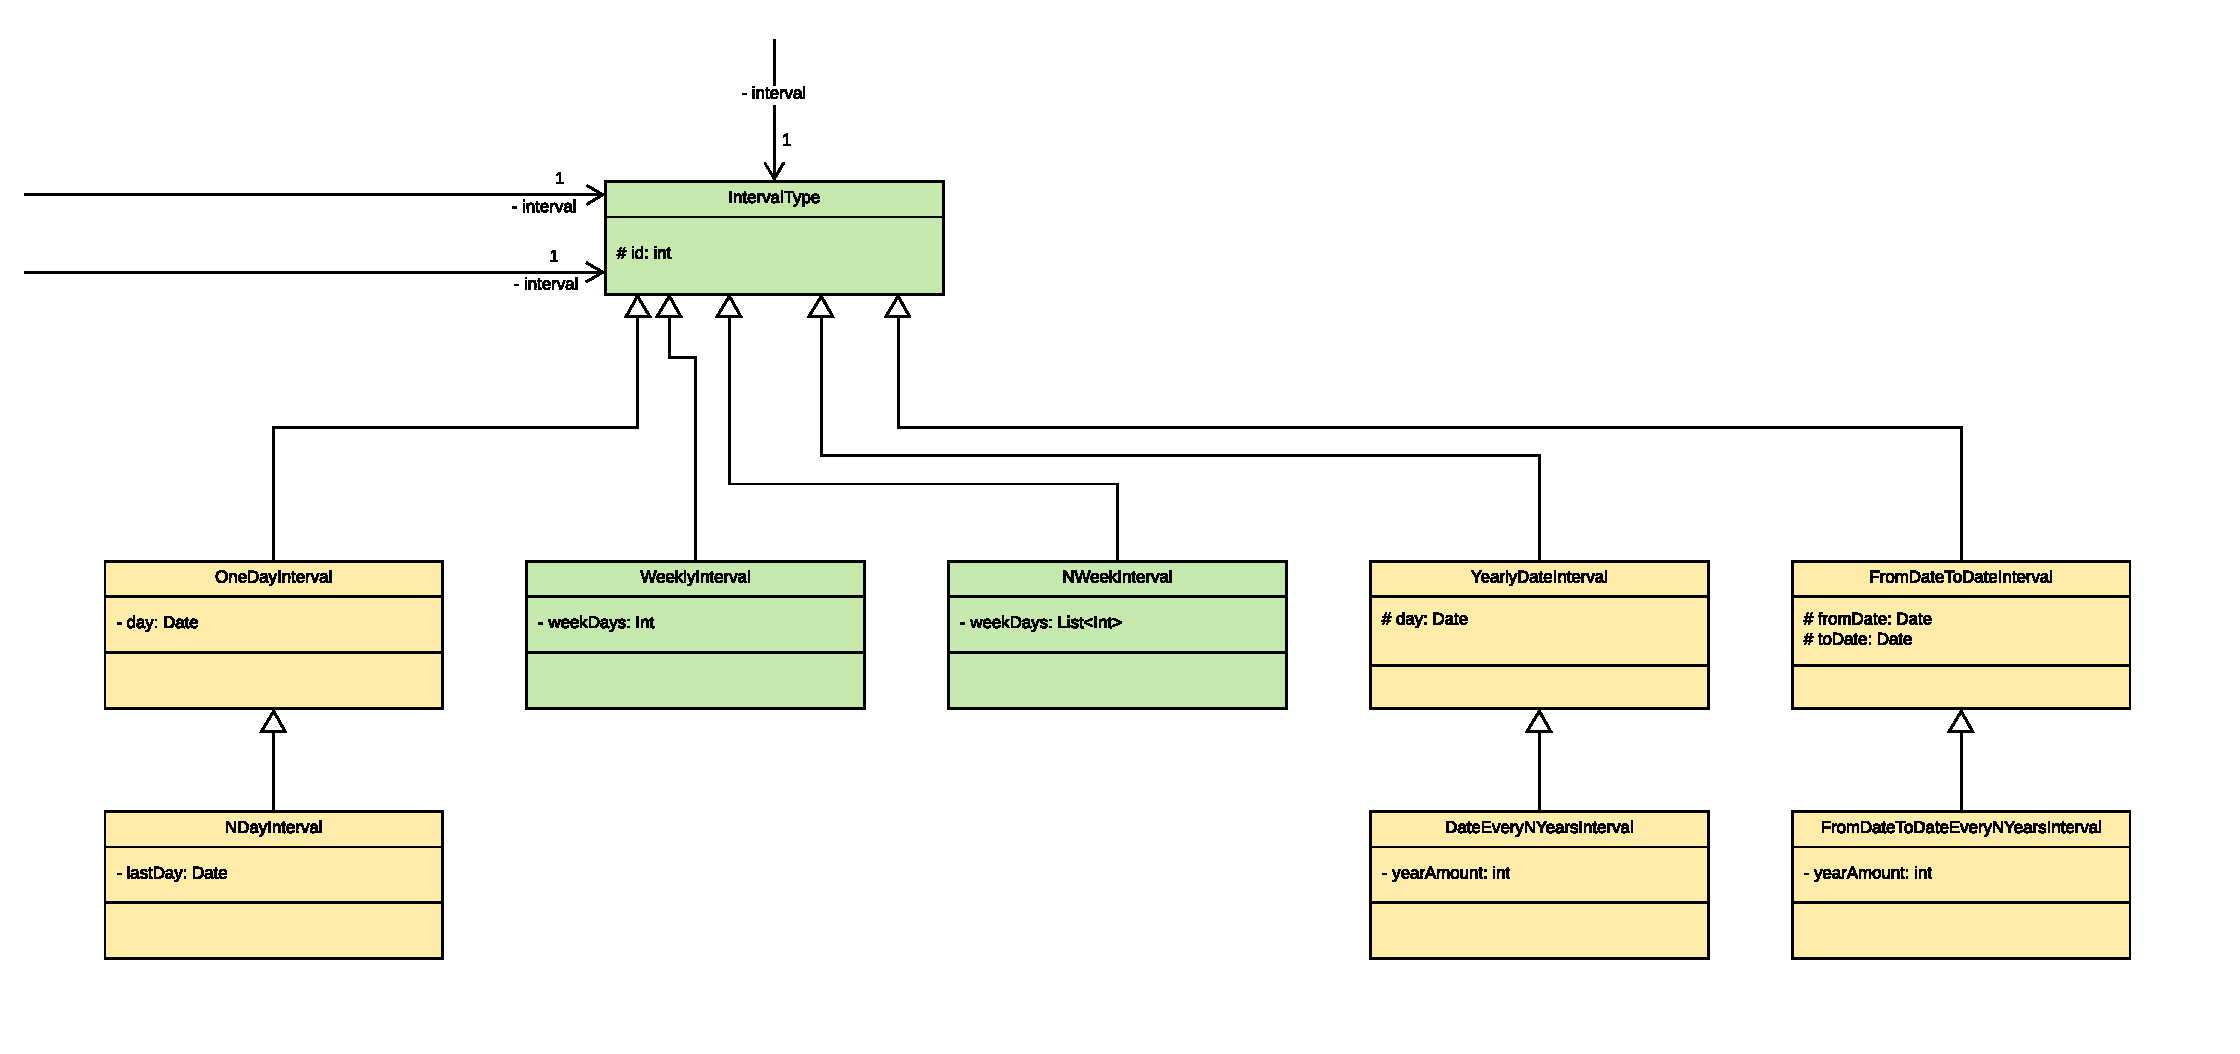
\includegraphics[width=1.0\textwidth]{pdfs/Interval1}
	        \caption[Současný návrh entity \texttt{Interval}]{Návrh entity \textit{Interval} podle doménovém modelu z předmětu BI-SP2}\label{image:Interval1}
        \end{figure}
        Prvním takovým požadavkem je změna entity \verb|Interval| (viz obrázek \ref{image:Interval1}), která je široce využívaná v projektu. Návrh řešení tohoto problému bude popsán v sekci \ref{navrh:upravy}. Tady bude popsán jenom problém samotný. Entita \verb|Interval| reprezentuje časové rozmezí pro pečovatelské dny, opakované události, nastavení alimentů a navazující se na ně požadavky na změny a historické záznamy.
            
        Jádro problému je v tom, že entita je navržena pomoci generalizace, neboli dědičnosti z hlediska implementace. Takový návrh dává možnost vytvořit konkretní typ intervalu pomocí zvolení odpovídající třídy. Na druhou stranu takový návrh působí komplikaci při implementace a současně nepokrývá všechny možné případy využití intervalů. Například, není možné sestavit interval, který se bude opakovat každý poslední den měsíce. Pokud bychom se chtěli držet aktuální implementaci a zároveň pokryt všechny možné případy, ztratili bychom přehlednost zvolení správné třídy při vytváření instance.
            
        Dalším problémem návrhu entity \verb|Interval| je provázanost s pečovatelskými dny. Při návrhu frontendové částí aplikace bylo zjištěno, že pečovatelské dny nepotřebují komplikované nastavení a zároveň by potřebovaly mít odkazy na konkretního rodiče, který je zodpovědný za dítěte v tento den nebo časový úsek. Proto je potřeba oddělit interval pečovatelských dnů zvlášť od ostatních intervalů
    
    \subsection{Alimenty}
        \begin{figure}\centering
	        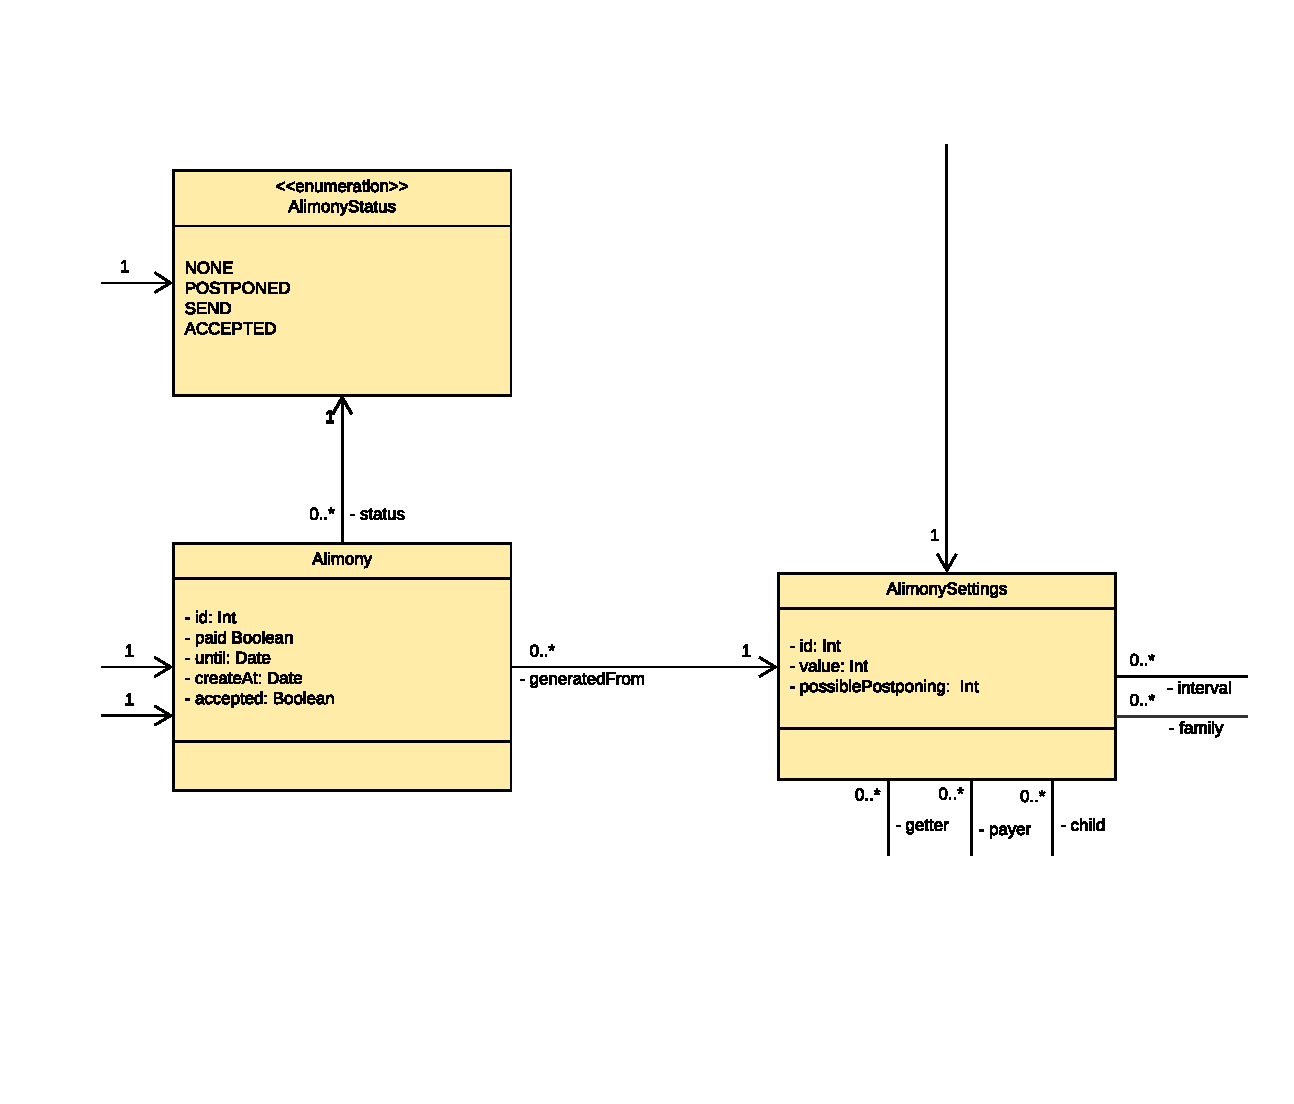
\includegraphics[width=0.9\textwidth]{pdfs/AlimonyDraft1}
	        \caption[Návrh entit \texttt{Alimony} a \texttt{AlimonySettings}]{Návrh entit \texttt{Alimony} a \texttt{AlimonySettings} podle doménového modelu z předmětu BI-SP2}\label{image:aliomny-draft1}
        \end{figure}
        Entita \verb|Alimony| reprezentuje alimenty, které jeden rodič má posílat druhému rodiči. Jedna instance se odpovídá alimentům za jeden měsíc. Současný návrh popisuje entitu a její navázanost na entitu \verb|AlimonySettings|(viz obrázek \ref{image:aliomny-draft1}). Nastavení alimentů definují dlouhodobou konfiguraci. Potom na základě této konfiguraci se vytváří jednotlivé instance alimentů. Nastavení se definují v rámci jedné rodiny. V případě potřeby, rodiče mají možnost rozdělit alimenty do několika nastavení, které budou současně validní.
        
        Hlavní problém je v tom, že instance alimentů by se měly vytvářet nezávisle na frontendové části aplikace, což není popsáno v současném návrhu aplikace. Podrobně návrh řešení problému bude popsán v sekci \ref{navrh:upravy:alimenty}.
        
        Dodatečným požadavkem frontendového týmu se týká entity \texttt{Alimony} samotné. Za účelem zjednodušení návrhu frontendové části aplikace, je potřeba přidat závislost na entitu \texttt{Family}. % V takovém pŕípade aplikace může ihned po nalazení novych alimentu rict uZivateli ktere rodine patri tyto alimenty.
        
    \subsection{Pečovatelské dny}\label{analyza:pozadavky:caredays}
        Než se zanořit do podrobného popisu problému, je potřeba popsat účel této entity a její využiti backendém a frontendém. Tato entita reprezentuje jednorázový interval nebo opakující se interval pečovatelských dnů jednoho z rodičů nebo ostatních členů rodiny. Pro rozlišování pečovatelských dnů různých členů rodiny každý uživatel má přiřazenou vlastní barvu. Tato entita se používá za dvěma účely. První a nejdůležitější účel je nastavení pečovatelských dnů pro rodiče. Nastavení musí pokrývat všechny dny kalendáře. Dítě by nemělo mít ve svém kalendáři den, který není označen žádnou barvou a zároveň by neměly vznikat konflikty. Druhým účelem jsou jednorázové změny pečovatelských dnů. Tyto změny jsou vyžadovány pro případy, kdy dlouhodobé nastavení kalendáře neplatí. Příkladem může být výlet dítěte k babičce a dědečkovi. Během tohoto časového intervalu rodiče nejsou zodpovědné za dítěte, proto je potřeba uvést jednorázovou změny do kalendáře, která zaznamená tuto situaci. Jiným příkladem je předání péče jednoho rodiče druhému, což se může nastat z různých důvodu.

        \begin{figure}\centering
            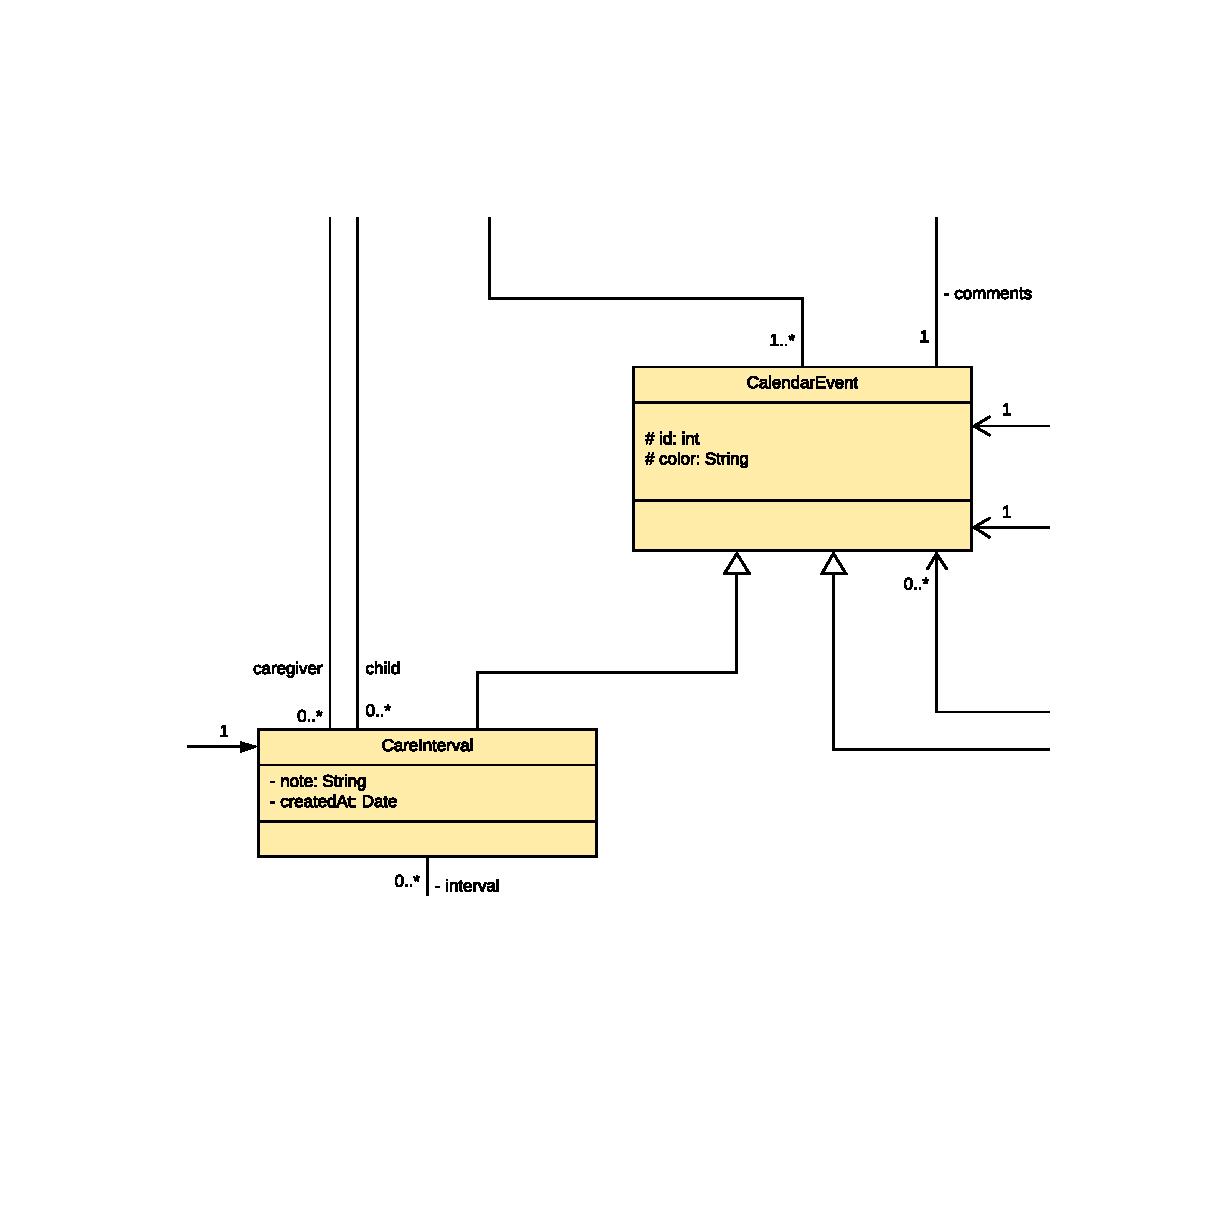
\includegraphics[width=0.8\textwidth]{pdfs/CareDays1}
            \caption[Současný návrh pečovatelských dnů]{Návrh pečovatelských dnů podle doménového modelu předmětu BI-SP2}\label{image:caredays1}
        \end{figure}
        Aktuální návrh pečovatelských dnů je navržen příliš komplikovaně (viz obrázek \ref{image:caredays1}) a zahrnuje dva různých případy využití. Dlouhodobá nastavení pečovatelských dnů rodičů nevyžadují komplikovaný návrh intervalů (viz sekci \ref{analyza:pozadavky-frontendu}), proto je potřeba oddělit řešení tohohle problému. Také je potřeba přidat odkaz na konkretního rodiče který je zodpovědný za tento den pro zjednodušení práce s touto entitou v rámci frontedové části aplikace. Jednorázové změny pečovatelských dnů je druhým problém, který je potřeba oddělit. Návrh této entity je podobnější aktuálnímu návrhu, protože tyto změny mohou vyžadovat složité pravidla opakování. Popis navržených změn a následné implementace bude popsán v sekci \ref{navrh:upravy:caredays}
        
     \subsection{Oznámení}
        \begin{figure}\centering
            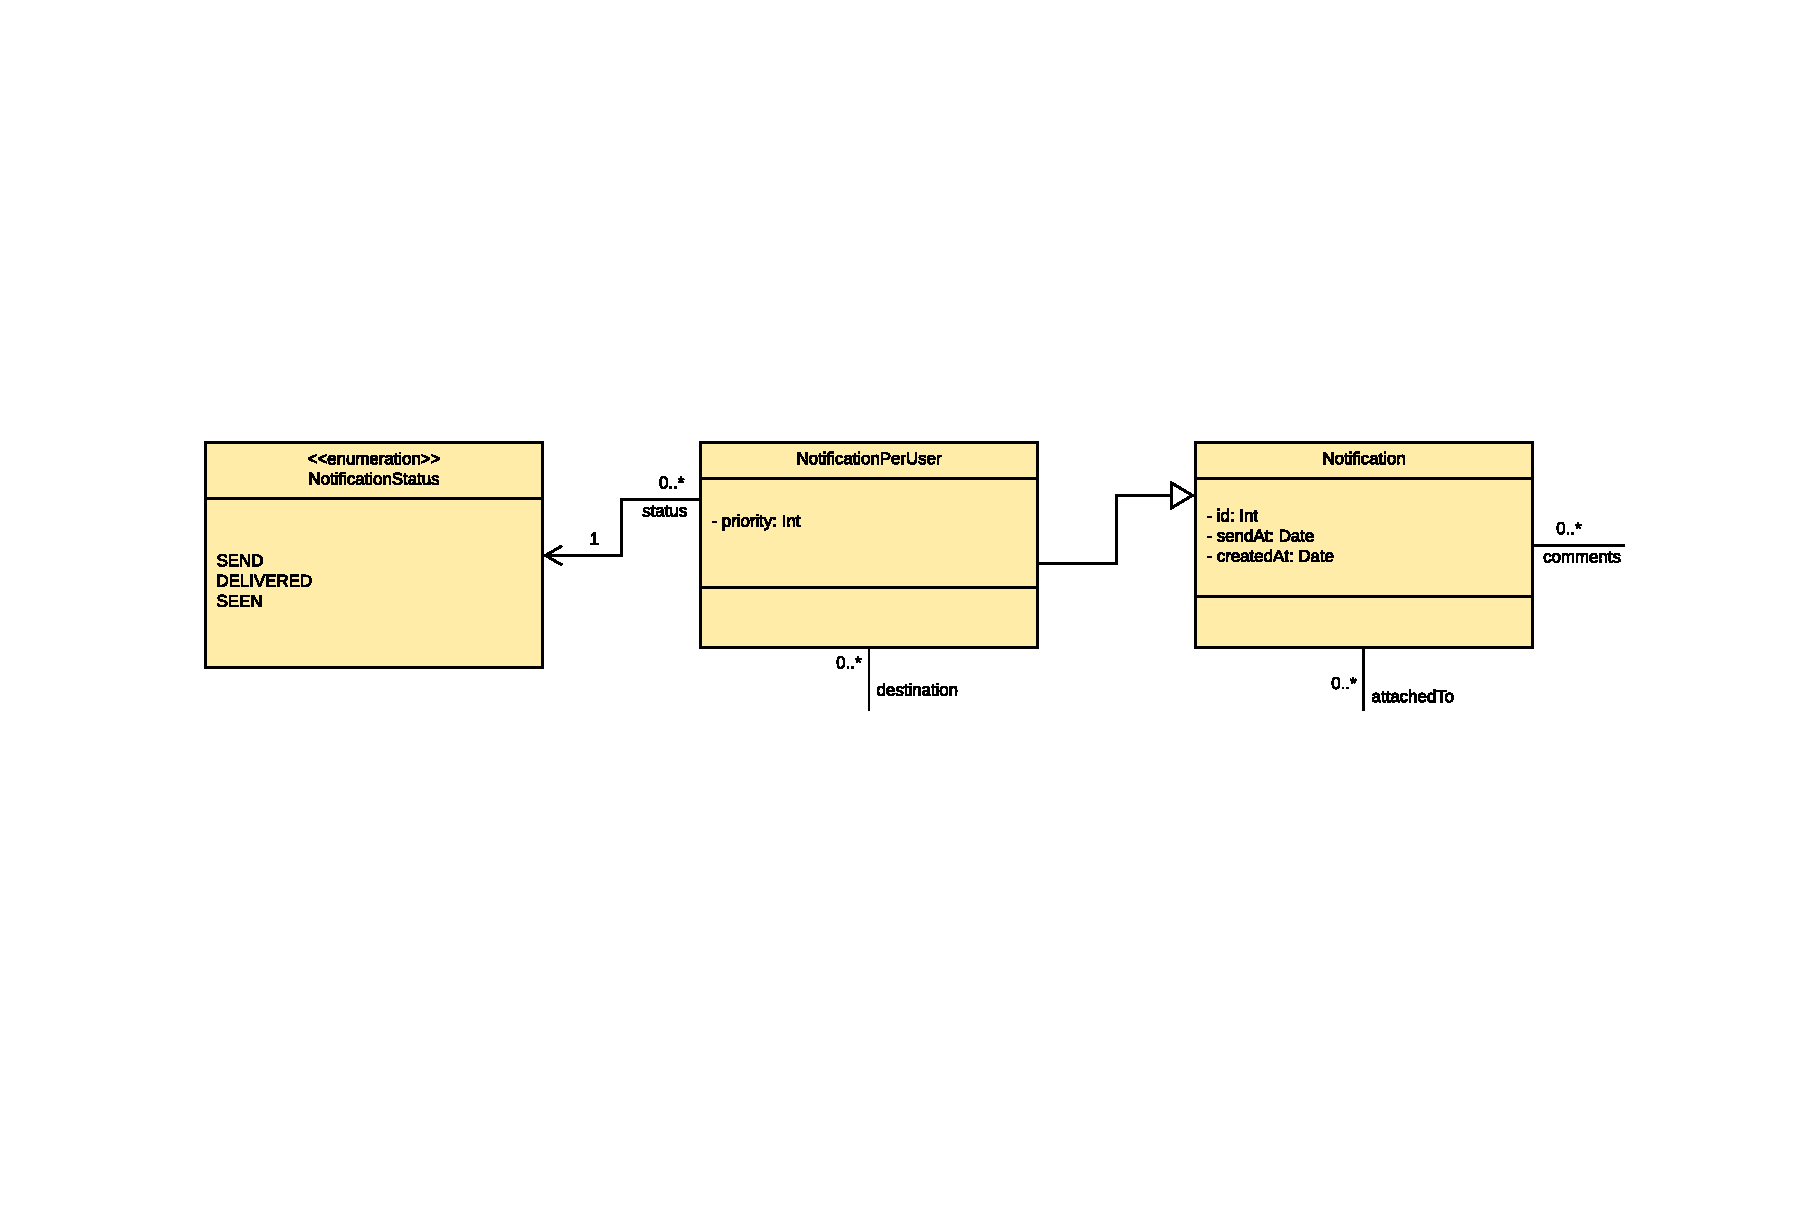
\includegraphics[width=1.0\textwidth]{pdfs/Notification1}
            \caption[Předchozí návrh oznámení]{Návrh oznámení podle doménového modelu předmětu BI-SP2}\label{image:notification1}
        \end{figure}
        Současný návrh oznámení (viz obrázek \ref{image:notification1}) reprezentuje upozornění uživatele o požadavku na změnu. Příčin oznámení uživatele ve skutečnosti je více:
        \begin{itemize}
            \item změny pečovatelských dnů;
            \item alimenty;
            \item změny nastavení alimentů;
            \item potřeby dítěte;
            \item změny v rámci rodiny.
        \end{itemize}
        Také frontendová část aplikace vyžaduje přizpůsobení oznámení upozorněním v rámci Android aplikace, což vyžaduje úpravu atributů. Také je potřeba specifikovat která událost způsobilá vytvoření tohoto oznámení a přidat typ této události podle výše uvedeného seznamu. Za účelem navrženi kvalitnějšího API je také potřeba přidat možnost přečíst všechny upozornění, které má uživatel, najednou. Řešení problému bude popsáno v sekci \ref{navrh:upravy:notification}.
        
            
            % reprezentuje libovolný typ oznámení. Tudíž oznámení pomocí elektronické pošty a pomocí upozornění v telefonu jsou reprezentovány pomocí stejné entity.
            
            % Frontedová část aplikace vyžaduje přizpůsobení oznámení upozorněním v rámci Android aplikace, což je konkretním typem oznámení a vyžadují sadu specifických atributu:
            % \begin{itemize}
            %     \item ID
            %     \item 
            % \end{itemize}
            % Řešení tohoto problému bude popsáno v sekci \ref{navrh:upravy:notification}
            
    % \section{Analýza konkurence}
    %     Tento návrh...
% \section{Analýza testování}

\section{Analýza bezpečnosti}
    V této sekci budou popsány procesy, které by měly zaručovat bezpečnost aplikace ze strany serverového backendu.
    
    \subsection{Role}\label{analyza:bezpecnost:role}
    
    % Aplikace je navržená tak, že první věc, kterou uživatel udělat, je registrace. Uživatel potřebuje zvolit jméno, příjmení, email a heslo. Na základě těchto údajů se vytváří účet uživatele. V Doménovém modelu tato třída se jmenuje \texttt{User}. V tento okamžik uživatel má role \texttt{USER}, která mu nadává možnost udělat jenom omezený počet věcí.  
        \begin{figure}\centering
	        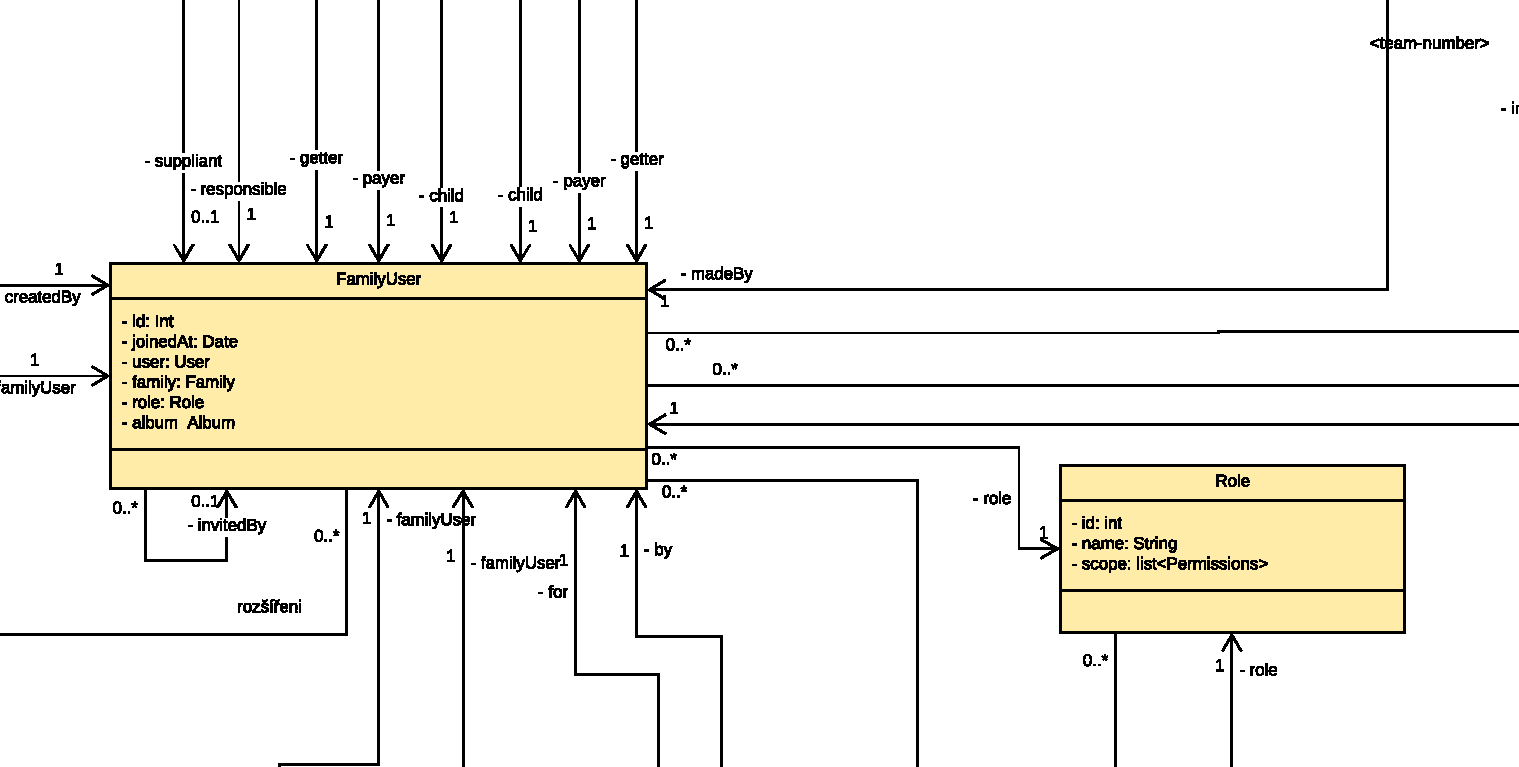
\includegraphics[width=1.0\textwidth]{pdfs/Role1}
	        \caption[Návrh \texttt{Role}]{Návrh entity \texttt{Role} podle doménového modelu z předmětu BI-SP2}\label{image:Role1}
        \end{figure}
        Než se uživatel přihlásí do rodiny, nemá žádnou roli. Po přihlášeni do rodiny, uživatel má roli v rámci přihlášené rodiny (viz obrázek \ref{image:Role1}), podle které mohou lišit jeho přístupová práva. Hlavní rolí v aplikace je rodič. Uživatel s takovou rolí má přístup ke všem potřebám dítěte a všem záznamem v kalendáři. Také, rodič může vytvářet pozvání do rodiny pro libovolného uživatele a nastavit mu libovolnou roli, včetně roli rodiče. Mimořádnou roli v rámci systému je dítěte. Uživatel s takovou rolí nemůže vlastnit pečovatelský den nebo splnit přání. Přihlášení dítěte muže proběhnout i bez vytvořeni klasického uživatele v rámci systému. Ostatní uživatele v rodině mají roli příbuzných. 
    
    \subsection{Autorizace}
        Návrh bezpečné aplikace nebyl cílem zmíněných v sekcích \ref{analyza:navrh:sp1} a \ref{analyza:navrh:sp2} předmětů. Proto návrh a současná implementace neobsahuje proces přihlašování uživatele do systému. Navržené procesy autentizaci a autorizaci budou podrobné popsány v sekci \ref{navrh:bezpecnost}.
        
\section{Analýza testování}\label{analyza:testovani}
    Současný návrh neobsahuje informaci o implementaci testování. Ale současná implementace obsahuje jeden test, který se zaměřuje na ověření, jestli se načetl {kontext aplikace}\footnote{Pokročilý kontejner, který funguje podobně \texttt{BeanFactory}. Načítá definice beanů, provazuje je a vydává v případe nutnosti} (viz obrázek \ref{code:test-context-loads1}).
    \begin{figure}
    \begin{minted}[frame=lines,
        framesep=2mm,
        baselinestretch=1.2,
        fontsize=\footnotesize,
        linenos]{java}
@RunWith(SpringRunner::class)
@SpringBootTest
class RozvodyApplicationTests {

    @Test
    fun contextLoads() {
    }

}
        \end{minted}
        \caption{Ukázka současného testování} 
        \label{code:test-context-loads1}
        \end{figure}
        
\section{Průběžná integrace}
    Na začátku je potřeba popsat pravidla zavedené pro distribuovaný systém správy verzí -- Git -- před začátkem implementace serveru. Proces vývoje byl rozdělen do dvou hlavních větví. První větev reprezentuje aktuální verzi aplikace a je označena jako \enquote{master}, což je implicitní větev v rámci Git. Druha větev je označena jako \enquote{dev} a určena pro proces vývoje. Pro implementaci jednotlivých úkolů je potřeba udělat kopii této větví a po vyřešení tohoto úkoly je potřeba zařadit všechny změny zpět do větví \verb|dev|. Takový přístup dává možnost pracovat na stejném projektu několika programátorům najednou a s jistotou uschovávat vlastní změny na server bez ohledu na jejích kompletnost.
    
    Vedoucím této bakalářské práce, a současně vedoucím tohoto projektu, byl poskytnout server pro testování, dostupný z IP: \enquote{http://37.46.80.230/}. Větve \verb|master| a \verb|dev| se automaticky nasazují po aktualizaci. Aplikace uložena do větvi \verb|master| je dostupná na portu 8998. Aplikace uložena do větvi \verb|dev| je dostupná na portu 8778.